\section{评价方法}

\subsection{论文中采用的评价方法}
文中采用{\color{blue}混淆矩阵(CM)}(混淆矩阵介绍见~\ref{CM})对分类器的分类效果进行评价。评价时计算的是CM的召回率(recall即the rate of true positives)和1-precision(low contamination即the rate of false positives)。

论文中的具体介绍:
\begin{tcolorbox}[colback=red!5,colframe=blue!75!black]
~~~~Evaluation of classifier performance requires the examination of a {\color{blue}Confusion matrix (CM)}, which is a contingency table crossing true (manually validated) and predicted (assigned by the classifier) identification of objects. Correct interpretation of the CM requires the examination of each category separately, including {\color{blue}the rate of true positives} as well as {\color{blue}false positives}.
\begin{itemize}
    \item the rate of true positives (recall)
        \begin{displaymath}
            true~positives=\frac{number~of~objects~correctly~predicted}{total~number~actual~objects}
        \end{displaymath}
    \item the rate of false positives (low contamination)
        \begin{displaymath}
            false~positives=\frac{number~of~objects~falsely~assigned~to~a~category}{total~number~of~predicted~objects}
        \end{displaymath}
\end{itemize}
\end{tcolorbox}

论文中的评价结果如图~\ref{fig:cmlearn}:
    \begin{figure}[!ht]
      \centering 
        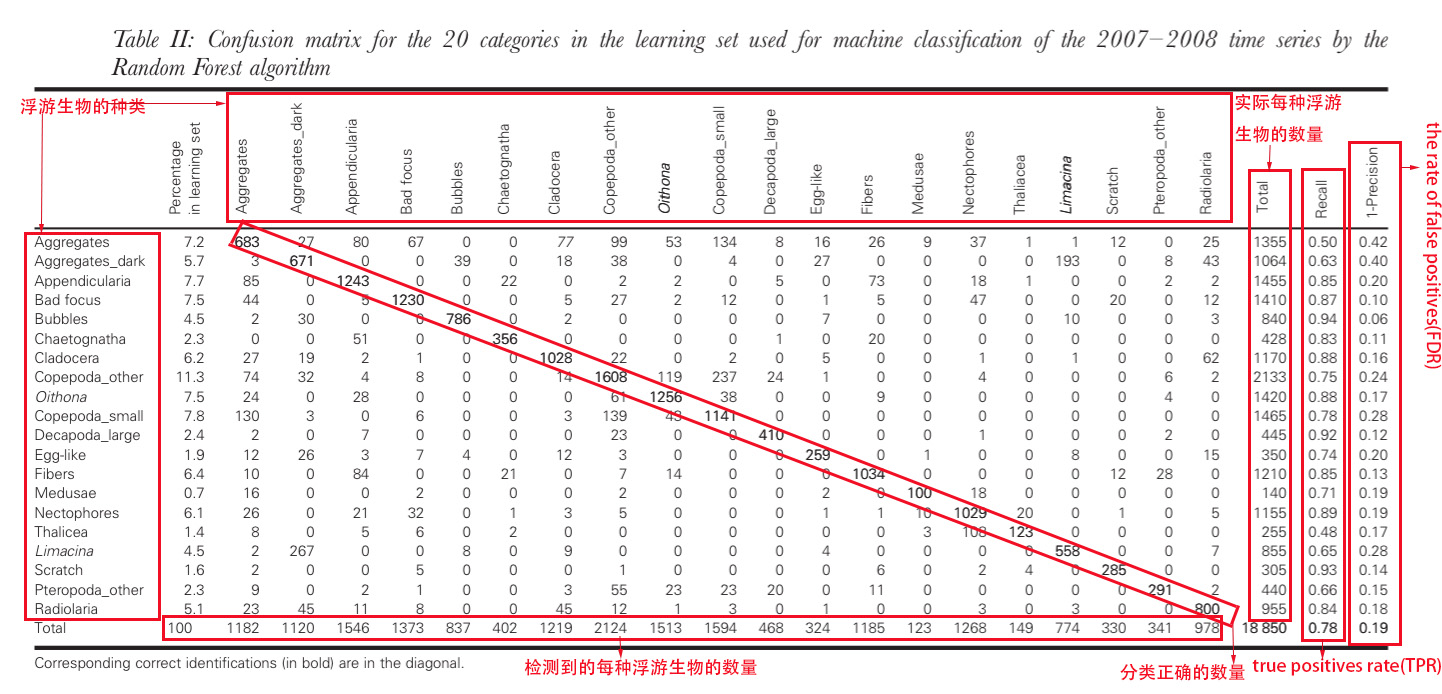
\includegraphics[width=1\textwidth]{cmlearn}
        \caption{Confusion matrix for the 20 categories in the learning set}
        \label{fig:cmlearn}
    \end{figure}
    
\subsection{怎样得到混淆矩阵}
论文中提到三种得到CM的方法(即采用什么训练集和测试集来生成):
    \begin{enumerate}
        \item Re-substitution CM
        
       这个方法是采用的测试集和训练集为同一个数据集。在这个过程中,用产生的分类器对测试集进分类时,得到的分类结果错误较少甚至可能没有错误,采用CM进行评价时就会低估分类器的错误率。
        \item Cross-validation CM
        
        这个方法是采用交叉验证(交叉验证介绍见\ref{cv})的方法。在这个过程中,将一个数据集分成n个相等的子集,用其中n-1个子集来训练产生分类器,用剩下的1个子集来进行测试,重复进行n次来构建CM。
        \item Uses two equivalent and independent learning files describing the same categories with different objects
        
        这种方法是用两个相等且相互独立的数据集分别作为训练集和测试集,根据测试结果建立CM。两个相等的数据集即在两个集合中浮游生物的种类相同,但是每种浮游生物中的个体是不同的。
    \end{enumerate}
    
\subsection{PkID中的评价参数}
PkID中通过5-折交叉验证 (介绍见\ref{kCM}) 得到混淆矩阵,对分类器进行评价。5-折交叉验证将数 据集分为 5 份,轮流将其中 4 份作为训练数据,1 份作为测试数据,进行试验。每次试验都会得出相 应的误分类率 (error rate 介绍见\ref{kCM}) 如图\ref{fig:five}。
    \begin{figure}[!ht]
      \centering 
        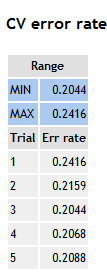
\includegraphics[width=0.1\textwidth]{five}
        \caption{5 次的误分类率}
        \label{fig:five}
    \end{figure}
    
    交叉验证得到的分类器总混淆矩阵(五次分类的累计结果)和误分类率(五次分类误分类率的平均值)如图\ref{fig:pkidCM}。
   \begin{figure}[!ht]
      \centering 
        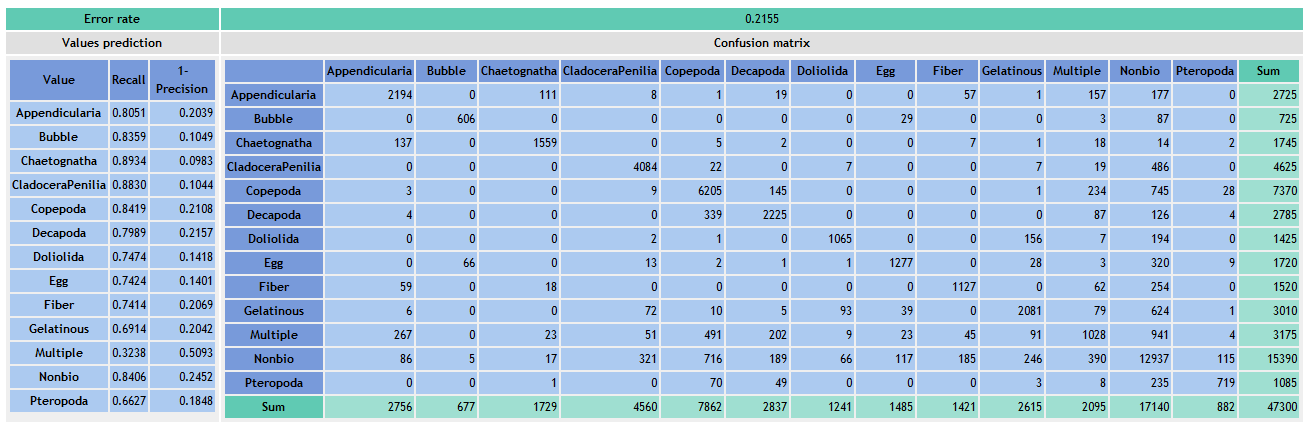
\includegraphics[width=1\textwidth]{pkidCM}
        \caption{交叉验证得到的总混淆矩阵和误分类率}
        \label{fig:pkidCM}
    \end{figure}
    

%    \begin{tcolorbox}[colback=red!5,colframe=blue!75!black]
%    There are three ways to build a CM, all available in PkID.
%    \end{tcolorbox}
    



\subsection{混淆矩阵Confusion matrix (CM)}
\label{CM}

在机器学习中,混淆矩阵(CM)是一种比较简单的对学习算法性能进行评价的评估准则,而且是大多数指标的基础。常用的算法评估准则有:Confusion Matrix、ROC、Lift、Gini、K-S等等。\newline

混淆矩阵 (CM)\footnote{\url{http://baike.baidu.com/view/2781781.htm}}\footnote{\url{http://en.wikipedia.org/wiki/Confusion_matrix}}:混淆矩阵是一种评估分类器可信度的方法。在图像精度评价中,主要用于比较分类结果和实际测得值,可以把分类结果的精度显示在一个混淆矩阵里面。特别用于监督学习,在无监督学习一般叫做匹配矩阵。

混淆矩阵是一个n行n列的矩阵,n代表类别的数量。矩阵的每一列代表预测的每一类的数量,每一行代表实际的每一类的数量。对角线上表示分类正确的每一类的数量。

例如:有150个样本数据,这些数据实际分为3类,每类50个。分类结束后得到的混淆矩阵如图\ref{fig:cm}。例如:第一行说明类1的50个样本有43个样本分类正确,5个错分为类2,2个错分为类3;第一列说明类1有43个样本分类正确,类2的2个样本被错分为类1,类3没有样本被错分为类1;对角线上的数据表示,类1、2、3分别有43、45、49个样本被分类正确。\newline
    \begin{figure}[!ht]
      \centering 
        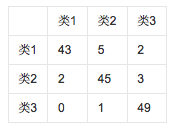
\includegraphics[width=0.3\textwidth]{cm}
        \caption{混淆矩阵例子}
        \label{fig:cm}
    \end{figure}

根据混淆矩阵可以导出以下几个参数\footnote{\url{http://www2.cs.uregina.ca/~dbd/cs831/notes/confusion_matrix/confusion_matrix.html}}:
\begin{itemize}
    \item true positives (TP):正样本被识别出的数量
    \item true negatives (TN):负样本被识别出的数量
    \item false positives (FP):负样本被错误分为正样本的数量
    \item false negatives (FN):正样本被错误分为负样本的数量\newline
    
    \item Accuracy:准确率,针对分类器的整个预测情况。
        \begin{displaymath}
            Accuracy=\frac{TP+TN}{TP+TN+FP+FN}
        \end{displaymath}
    \item {\color{red}Error rate:误分类率,针对分类器的整体预测情况。}(PkID 中使用的评价参数)
        \begin{displaymath}
            Error rate=\frac{FP+FN}{TP+TN+FP+FN}
        \end{displaymath}
    \item {\color{blue}The true positive rate (TPR) :召回率,就是正样本被识别出的概率。}(文中和PkID中使用的评价参数)
        \begin{displaymath}
            TPR=\frac{TP}{TP+FN}
        \end{displaymath}
     \item The false positive rate (FPR):虚警率,负样本被错误分为正样本的概率。
        \begin{displaymath}
            FPR=\frac{FP}{FP+TN}
        \end{displaymath}
    \item The true negative rate (TNR):负样本被识别出的概率
        \begin{displaymath}
            TNR=\frac{TN}{FP+TN}
        \end{displaymath}

    \item The false negative rate (FNR) :漏警率,正样本被错误分为负样本的概率。
        \begin{displaymath}
            FNR=\frac{FN}{FN+TP}
        \end{displaymath}
    \item {\color{blue}False discovery rate (FDR):1-precision。}(文中和 PkID 中使用的评价参数)
        \begin{displaymath}
            FDR=\frac{FP}{FP+TP}
        \end{displaymath}
    \item Positive predictive value (PPV)
        \begin{displaymath}
            PPV=\frac{TP}{TP+FP}
        \end{displaymath}
    \item Negative predictive value (NPV)
        \begin{displaymath}
            NPV=\frac{TN}{TN+FN}
        \end{displaymath}
    
\end{itemize}

\begin{figure}[!ht]
\centering
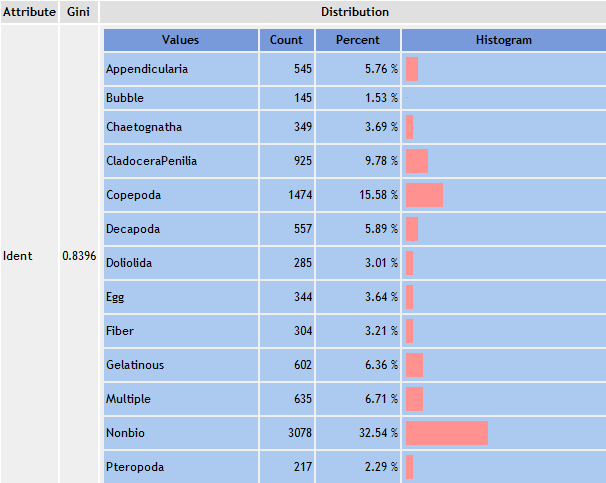
\includegraphics[width=0.8\textwidth]{每个类别所占比例.png}
\caption{数据集中每种类别的数目及所占比例}
\label{fig: ratio}
\end{figure} 

\subsection{交叉验证Cross Validation (CV)}
\label{cv}
交叉验证是用来验证分类器的性能一种统计分析方法,基本思想是把在某种意义下将原始数据进行分组,一部分做为训练集(training set),另一部分做为验证集(validation set),首先用训练集对分类器进行训练,在利用验证集来测试训练得到的模型,以此来做为评价分类器的性能指标。
\subsubsection{训练集和测试集}

在模式识别与机器学习的相关研究中,经常会将数据集分为训练集跟测试集这两个子集,前者用以建立模型,后者则用来评估该模型对未知样本进行预测时的精确度,正规的说法是泛化能力。怎么将完整的数据集分为训练集跟测试集,必须遵守如下要点:
\begin{enumerate}
    \item 只有训练集才可以用在模型的训练过程中,测试集则必须在模型完成之后才被用来评估模型优劣的依据。
    \item 训练集中样本数量必须够多,一般至少大于总样本数的50\%。
    \item 两组子集必须从完整集合中均匀取样。
\end{enumerate}

        {\color{blue}注:}其中最后一点特别重要,均匀取样的目的是希望减少训练集和测试集与完整集合之间的偏差,但却也不易做到。一般的作法是随机取样,当样本数量足够时,便可达到均匀取样的效果,然而随机也正是此作法的盲点,也是经常是可以在数据上做手脚的地方。举例来说,当辨识率不理想时,便重新取样一组训练集和测试集,直到测试集的识别率满意为止,但严格来说这样便算是作弊了。
        
        在MATALB中使用cvpartition对数据集进行随机拆分,完成交叉验证。
        
\subsubsection{常见的交叉验证方法}

\begin{itemize}
    \item Hold-Out Method
    
    将原始数据随机分为两组,一组做为训练集,一组做为验证集。
    \item Double Cross Validation(2-fold Cross Validation,记为2-CV)
    
    将数据集分成两个相等大小的子集,进行两回合的分类器训练。在第一回合中,一个子集作为training set,另一个便作为testing set;在第二回合中,则将training set与testing set对换后,再次训练分类器。
    {\color{blue}\item K-fold Cross Validation(K-折交叉验证,记为K-CV)}(实验中采用的交叉验证方法)
    \label{kCM}
    将原始数据分成K组,将每个子集数据分别做一次验证集,其余的K-1组子集数据作为训练集,这样会得到K个模型,用这K个模型最终的验证集的分类准确率的平均数作为此K-CV下分类器的性能指标。K一般大于等于2,实际操作时一般从3开始取。
    \item Leave-One-Out Cross Validation(记为LOO-CV)
    
    将每个样本单独作为验证集,其余的N-1个样本作为训练集,所以LOO-CV会得到N个模型,用这N个模型最终的验证集的分类准确率的平均数作为此下LOO-CV分类器的性能指标。相比于前面的K-CV,LOO-CV有两个明显的优点:
    \begin{itemize}
        \item 每一回合中几乎所有的样本皆用于训练模型,因此最接近原始样本的分布,这样评估所得的结果比较可靠。
        \item 实验过程中没有随机因素会影响实验数据,确保实验过程是可以被复制的。
    \end{itemize}
\end{itemize}
